\section{Avantages du traitement des données}
\paragraph{}
Le traitement des données est important pour de multiples raisons.
Premièrement, il est important d'éliminer le bruit ou tout type d'information non essentielle des données.
Deuxièmement, nous pouvons examiner comment nous pouvons tirer davantage d'informations de nos ``données brutes''.
% Data processing is important because of multiple reasons.
% First, it is important to remove noise or any kind of unessential information from or data.
% Secondly, we can look into how we can derive more information from our ``raw data''

\section{Travailler uniquement avec les yeux}
\label{data-processing:eyes}
\paragraph{}
Dans certaines des expériences suivantes, je me suis concentré sur l'extraction des yeux d'une image.
Pour cela, j'ai utilisé deux bibliothèques: dlib et imutils.
Sur la base des repères faciaux présentés dans l'introduction \ref{figure:facial-landmarks}, j'ai extrait uniquement la partie de l'image décrite par les repères faciaux pour les yeux.
% In some of the following experiments, I focused on only extracting the eyes from an image.
% For this, I used two libraries: dlib and imutils.
% Based on the facial landmarks that were presented in the introduction \ref{figure:facial-landmarks}, I extracted only the image portion described by the facial landmarks for the eyes.

\begin{lstlisting}[language=Python, caption=Extraire le contour des yeux]
class FaceDetector(metaclass=Singleton):
    def __init__(self):
        self._face_detector = dlib.get_frontal_face_detector()
        self._face_predictor = dlib.shape_predictor(
            Config.face_landmarks_path)

    def get_eye_contours(self, cv2_image):
        """Returns a list of eye contours from a cv2_image. First contour is for the left eye"""
        contours = []
        gray_image = Utils.convert_to_gray_image(cv2_image)
        rects = self._face_detector(gray_image, 0)
        if len(rects) > 0:
            # only for the first face found
            shape = self._face_predictor(gray_image, rects[0])
            shape = face_utils.shape_to_np(shape)
            (left_eye_start,
             left_eye_end) = face_utils.FACIAL_LANDMARKS_IDXS["left_eye"]
            (right_eye_start,
             right_eye_end) = face_utils.FACIAL_LANDMARKS_IDXS["right_eye"]
            contours.append(shape[left_eye_start:left_eye_end])
            contours.append(shape[right_eye_start:right_eye_end])
        return contours
\end{lstlisting}

\clearpage
\paragraph{}
Comme nous ne nous intéressons qu'au contraste entre l'iris et la pupille, j'ai ensuite appliqué un \emph{seuil binaire} sur l'image grise de l'œil pour souligner la façon dont la pupille est située par rapport à l'ensemble de l'œil.
% Since we are only interested in the contrast between the iris and the pupil, I afterwards applied a \emph{binary threshold} on the eye's gray image to emphasize on how the pupil is situatied relative to the whole eye.

\begin{lstlisting}[language=Python, caption=Application d'un seuil binaire]
def get_binary_thresholded_image(cv2_image):
    img = convert_to_gray_image(cv2_image)
    img = cv2.medianBlur(img, 5)
    img = cv2.adaptiveThreshold(
        img, 255, cv2.ADAPTIVE_THRESH_GAUSSIAN_C, cv2.THRESH_BINARY, 11, 2)
    return img
\end{lstlisting}

\begin{figure}[H]
    \centering
    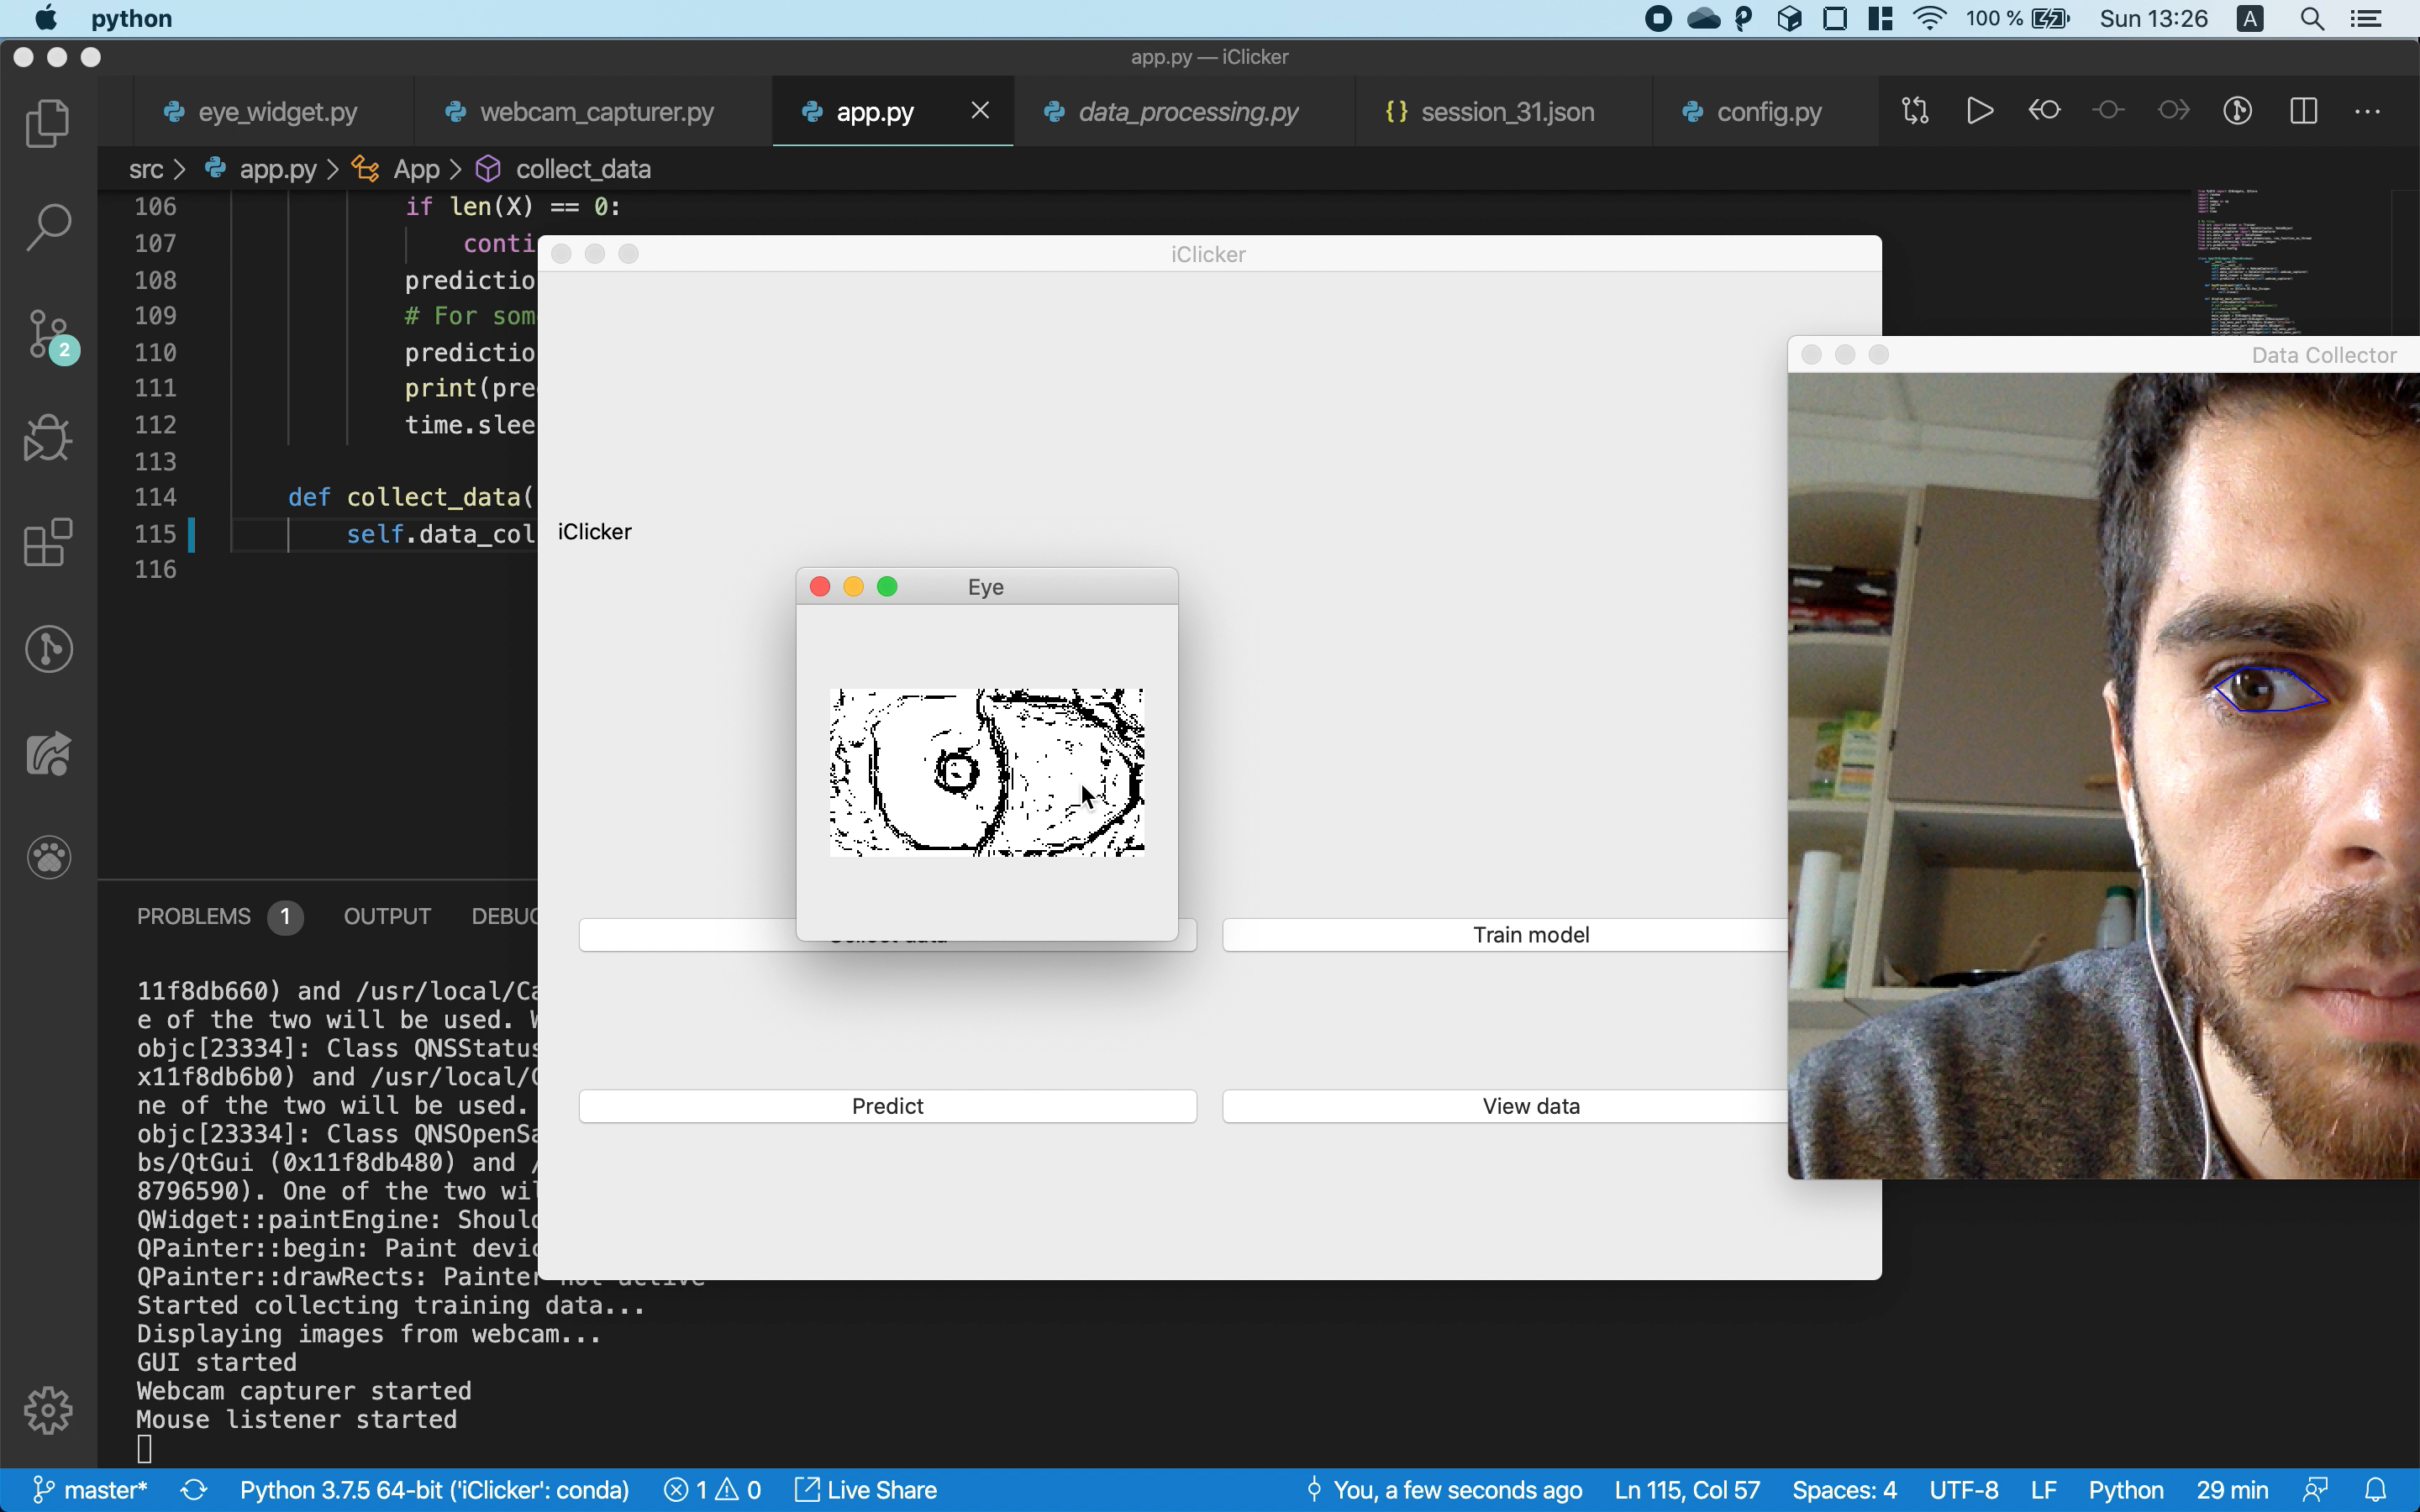
\includegraphics[width=\textwidth]{eye_binary_threshold.png}
    \caption{Obtenir des données sur les yeux}
\end{figure}

\section{En utilisant seulement le visage}
\paragraph{}
Un travail en cours porte sur la façon dont je peux utiliser le visage entier comme intrant pour un Réseau Neuronal Convolutif et sur la question de savoir si je dois y appliquer un traitement quelconque.
Je reviendrai lorsque j'aurai des résultats à ce sujet, car il s'agit d'un travail en cours.
% A current work in progress is researching on how I can use the whole face as an input for a Convolutional Neural Network and whether I should apply any kind of processing to it or not.
% I will come back when I have some results for this, as this is work in progress.

